% vim: set tw=0:
\documentclass{beamer}
\usepackage{graphicx}

% Reasonable themes:
% Antibes Bergen Berkeley Berlin Frankfurt Goettingen Ilmenau Luebeck Malmoe
% Montpellier PaloAlto Rochester Singapore Szeged Warsaw bars boxes
% compatibility default lined plain shadow sidebar split tree
% And these ones include the author's name on every slide:
% Berkeley

% Declare themes.
\mode<presentation>
\usetheme{UWHEP}

% Personal macros.
\newcommand{\email}[1]{{\texttt #1}}
\newcommand{\newframe}[1]{\section{#1}
    \frametitle{\sc{#1}}}
\newcommand{\subframe}[1]{\subsection{#1}
    \frametitle{\sc{#1}}}
\newcommand{\supers}[1]{\ensuremath{^\textrm{#1}}}
\newcommand{\subs}[1]{\ensuremath{_\textrm{#1}}}
\newcommand{\ca}{\ensuremath{\sim}}

% Author information.
\title{T2 Status}
\author[Maier, Mohapatra]{
    Will Maier \and Ajit Mohapatra\\ 
    {\tt wcmaier@hep.wisc.edu}\\
    {\tt ajit@hep.wisc.edu}}
\institute[Wisconsin]{University of Wisconsin - High Energy Physics}
\date{2008.06.10}
\logo{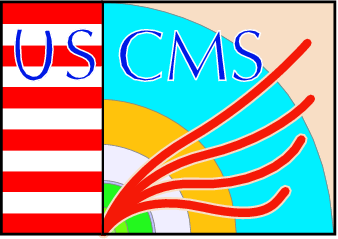
\includegraphics[height=0.6cm]{../../../Graphics/USCMS_logo.png}\hspace{.1cm}
\includegraphics[height=0.75cm]{../../../Graphics/UW_logo.png}}

\begin{document}

\begin{frame}
    \titlepage
\end{frame}

%\section{Overview}
%\begin{frame}
%    \tableofcontents
%\end{frame}

% http://indico.cern.ch/conferenceDisplay.py?confId=35597
% +1 626 395 2112 / 383891
\section{Facilities}
\subsection{Software and Storage}
\begin{frame}
\frametitle{}
\begin{itemize}
    \item NFSlite deployment successful
    \begin{itemize}
        \item Two CRAB-related AFS outages; impossible to keep up with new bugs/features
        \item Sent in fix for bug in new CRAB that breaks on NFSlite-like setups
        \item Improved AFS stability -- no issues since deployment
    \end{itemize}
    \item Debugged bad routing between Wisconsin and FNAL
    \begin{itemize}
        \item Switched to new fiber path at Wisconsin
        \item Ajit noticed lower PhEDEx transfer peaks from FNAL
        \item Routed over ESnet; FNAL fixed BGP advertisement
    \end{itemize}
    \item Installed new RSV
    \begin{itemize}
        \item Doing well since the switch
    \end{itemize}
    \item Installing gLexec
    \begin{itemize}
        \item Complicated by AFS, absolute links, hardcoded rpaths and 32 vs 64 bit clients
        \item It'd be great if wnclient/pacman weren't so fragile after install (and could be moved without breaking updates)
    \end{itemize}
\end{itemize}
\end{frame}

\subsection{Production and Monitoring}
\begin{frame}
\frametitle{}
\begin{itemize}
    \item SAM: OK
    \item JobRobot: OK 
    \item PhEDEx:
    \begin{itemize}
        \item All 8 commissioned links from T1 to Wisconsin were exercised successfully in the Prod instance during CCRC
        \item Lots of CCRC analysis
        \item Hosting CSA08 datasets for post-CCRC user analysis
    \end{itemize}
    \item MC Production:
    \begin{itemize}
        \item Waiting for 2\_1\_x release for the next round of production
    \end{itemize}
\end{itemize}
\end{frame}

\end{document}
